\cleartooddpage[\thispagestyle{empty}]

\newcommand{\Lim}[1]{\raisebox{0.5ex}{\scalebox{0.8}{$\displaystyle \lim_{#1}\;$}}}

\chapter{Gamma Rays and Dark Matter}\label{ch_gamma}


This analysis searches for dark matter using gamma rays, thus a discussion on gamma rays and their properties is necessary.
In this chapter, three different topics are discussed.
The first is the astrophysical mechanisms that produce gamma rays, the second is how dark matter around the Galactic Center can produce gamma rays, and the third is how gamma rays induce air showers in the Earth's atmosphere.

\section{Production of TeV Gamma Rays}

  There are several mechanisms that can produce photons with TeV energies.
  A gamma ray can start as a low-energy photon, then gain significant energy from electroweak interactions with electrons, referred to as a leptonic production.
  Alternately, a gamma ray can be created from a high-energy proton colliding with another proton, referred to as hadronic production.
  The primary mechanism this analysis searches for is the annihilation of two WIMP dark matter particles that either directly or indirectly produce gamma rays, and is discussed in Section~\ref{dm_spectral}.

  In leptonic production, electrons and low-energy photons collide, transferring energy to the photon.
  This interaction is called upscattering or Inverse Compton scattering~\cite{compton_effect}.
  In Inverse Compton scattering, a charged particle interacts with a photon, and some the electron's kinetic energy is transferred to the photon, shifting it to a higher frequency.
  {\color{red}(This is a good example where physics details are needed. Even if it does not pertain directly to the signal you are looking for, you have to explain here what IC is. Show the Feynman diagram, maybe the cross-section, describe a little better/longer. Also, how are the low energy photons produced?? -Orel)}
  %While the chance that any one thermal photon will be upscattered to TeV energies is low, astrophysical scales involve large populations of photons and electrons.
  %When these two populations interact, a small fraction of the original photon population can achieve TeV-scale energies~\cite{gammas_from_electrons}.

  \begin{figure}[ht]
    \centering
    \includegraphics[width=0.45\textwidth]{images/feynman_particles/inversecompton.pdf}
    \caption[Inverse Compton Scattering Feynman Diagram]{
      Feynman diagram of Inverse Compton scattering.
    }
    \label{fig:inv_compt_feyn}
  \end{figure}

  In order to efficiently produce gamma rays via this method, a population of high-energy electrons is needed.
  One environment for producing these electrons is around pulsar wind nebulae.
  Due to their rapid rotation, pulsar wind nebulae are constantly twisting their magnetic field lines.
  These magnetic field lines get twisted tighter and tighter, until they break and reconnect with neighboring lines.
  This breaking and reconnection temporarily creates electric fields that can accelerate electrons outwards to higher energies than thermal sources (i.e. solar wind) alone can achieve~\cite{gamma_pwn1,gamma_pwn2}.
  {\color{red}(This paragraph also reads like a story and less like an accurate physical description. It should be rewritten more accurately. If you want, you can take the highlights from ref "Rees and Gunn, 1974" and rewrite them here. Or find a more modern paper/book to get a clearer description. -Orel ??)}

  Another mechanism that produces high-energy charged particles is located at supernova shockfronts, called diffuse shock acceleration~\cite{dsa1,dsa2,dsa3,dsa4,dsa5}.
  During and after a supernova's initial detonation, charged fermions are quickly heated.
  These heated particles then expand outwards, creating a moving shockfront at the boundary between the expanding particles and the surrounding Inter-Stellar Medium (ISM).
  These expanding particles bring their own magnetic fields, which can reflect charged particles.
  As the shockfront expands, it also runs into the ambient magnetic fields in the ISM, which can also reflect charged particles.
  This shockfront is shown in Figure~\ref{fig:snr_shockfront}.
  {\color{red}(Maria already mentioned it, and I agree, you need to provide the equations describing Fermi acceleration. Being more accurate about the fractions of particles reflected/accelerated, would be better as well. Essentially same as before, less story-like. Also, you speak in the paragraph about charged particles in general, but later you mention that this is a way to accelerate electrons. Maybe make it clearer?? -Orel )}
  
  \begin{figure}[ht]
    \centering
    \includegraphics[width=0.75\textwidth]{images/snr_shockfront/shockfront_diagram.pdf}
    \caption[Supernova Shockfront]{
      Diagram of supernova shockfront.
      Relative to some inertial observer, the supernova plasma expands at velocity $v_s$, while the ISM moves at velocity $v_m$.
    }
    \label{fig:snr_shockfront}
  \end{figure}
  
  In this situation, particles that are able to cross the shockfront are reflected off the magnetic fields on the other side, gaining a small amount of energy each time.
  On average, a particle gains energy for each crossings cycle (up-to-down and down-to-up stream) by Equation~\ref{eqn:snr_en_per_cycle}.
  
  \begin{equation}\label{eqn:snr_en_per_cycle}
    \left \langle \frac{\Delta E}{E} \right \rangle = \frac{4}{3} \left ( \frac{v_{s}-v_{m}}{c} \right )
  \end{equation}
  
  In Equation~\ref{eqn:snr_en_per_cycle}, $\Dela E$ is the energy gained by the particle, $E$ is the initial energy of the particle, $v_s$ is the velocity of the supernova expansion, and $v_m$ is the velocity of the ISM.

  Equation~\ref{eqn:snr_spectrum} shows the differential energy spectrum produced by particles that escape the shockfront.
  
  \begin{equation}\label{eqn:snr_spectrum}
    N(E)=E^{ \frac{log\:P}{log\: \beta} -1}
  \end{equation}

  Probability $P$ is the chance a particle is trapped between the shockfronts, calculated as $1 - \frac{R_o}{R_i}$, where $R_i$ is the rate initial particles are injected into the shockfront, and $R_o$ is the rate particles permanently escape downstream.
  The variable $\beta$ is the percent increase in energy during each crossing cycle, $\beta = 1+ \frac{4}{3} \left ( \frac{v_s - v_m}{c} \right )$.
  Since the trapping probability is less than 1 but also close to 1, for extremely small $P$'s, Equation~\ref{eqn:snr_simple_P} simplifies Equation~\ref{eqn:snr_spectrum} exponent numerator to -1.
  
  \begin{equation}\label{eqn:snr_simple_P}
    \Lim{P \rightarrow 1^{-}} \; \textrm{log}_{10} P = -P
  \end{equation}
  
  Likewise, since $\beta$ is greater than 1 but also close to 1, Equation~\ref{eqn:snr_simple_B} simplifies Equation~\ref{eqn:snr_spectrum} exponent denominator to 1.

  \begin{equation}\label{eqn:snr_simple_B}
    \Lim{\beta \rightarrow 1^{+} } \; \textrm{log}_{10} \beta = \beta
  \end{equation}
  
  {\color{red} Need to show why P and $\beta$ approach -1 and 1 ??}
  
  Since both $P$ and $\beta$ are close to -1 and 1 respectively, Equation~\ref{eqn:snr_spectrum} simplifies to $N(E) \approx E^{-2}$, matching the observed cosmic ray spectrum~\cite{}
  
  In Equation~\ref{eqn:snr_spectrum}, the exponent is often referred to as the spectral index $\gamma$.
  The spectral index's dependence on $P$ and $\beta$ is shown in two plots in Figure~\ref{fig:snr_spectrum}.
  The top plot in Figure~\ref{fig:snr_spectrum} shows how changing $\beta$, the energy gain per shockfront crossing cycle, and the bottom plot shows the differential spectra with the spectral indicies from the top plot.
  From these two plots, it can be seen that increasing the energy gain per crossing cycle $\beta$ creates a harder spectrum of particles with more higher energy particles, since they can reach escape energies in fewer cycles.
  It can also be seen that trapping more particles at the shockfront (higher $P$) also creates a harder spectrum of escaping particles, as particles can be contained for more cycles, gaining more energy before escaping~\cite{dsa6}.

  \begin{figure}[ht]
    \centering
    \includegraphics[width=0.8\textwidth]{images/snr_shockfront/snr_spectrum.pdf}
    \caption[Supernova Diffuse Acceleration Spectral Indicies]{
      The top plot shows the spectral indicies produced by various combinations of $\beta$, the fractional energy gained by a particle in one crossing cycle (upstream $\rightarrow$ downstream $\rightarrow$ upstream), and $P$, the average chance a particle isunable to escape the shockfront.
      The contours for three spectral indicies $\gamma$ are shown.
      For example, at the orange triangle, each crossing cycle increases a particles energy by a factor of 1.10, while it has a 90\% chance of being permanently trapped, which produces particles with a spectral index of $\gamma=-2.1$.
      The bottom plot shows the differential flux produced by power laws with the three spectral indicies shown in the top plot.
    }\label{fig:snr_spectrum}
  \end{figure}
  
  \FloatBarrier


  {\color{red}A fraction of the charged particles (What is the limit? When can they cross the shock front?? -maria)} in the expanding gas are able to cross the shockfront, where a small fraction will be reflected by magnetic fields.
  
  % slides on supernova shockwaves
  % https://isapp2012paris.sciencesconf.org/conference/isapp2012paris/Stefano_Gabici_three.pdf
  
  % Drury, 2012, "Origin of Cosmic Rays"
  % https://doi.org/10.1016/j.astropartphys.2012.02.006
  % Diffusive shock acceleration, 
  
  % https://www.annualreviews.org/doi/pdf/10.1146/annurev.aa.22.090184.002233 , pg 435:
  %   2 shockfronts, travelling at v1 and v2= v1 * 3/4
  %   v1 = B1 * c # velocity of the collisionless shockfront (just the B fields)
  %   v2 = B2 * c # velocity of the gas particles
  %   1 crossing cycle = reflect off each shock once = E * B2 * 4/3 increase in particle energy
  %   particle tends to escape after (B1-B2)*1/4 crossing cycles
  
  {\color{red}(specify that the particles have to be going faster than the shockfront??)}
  Upon recrossing the shockfront, they are again reflected by magnetic fields, which are expanding outwards with the supernova remnant gas, {\color{red}imparting energy (whats the formula for calculating this energy?? -maria)} to the charged particles.
  {\color{red}(relate this to how it contributes to the VERITAS background, since my DM signal doesn't come from fermi acceleration??)}
  These particles repeatedly cross the shockfront, where a smaller and smaller fraction of particles gain more and more energy, in a mechanism called first-order Fermi acceleration~\cite{fermi1949,highenergyelectron_snr}.
  While this acceleration mechanism can produce high-energy charged particles, its still uncertain as to how the initial particles gain the energy necessary to cross the shockfront, known as the injection problem~\cite{inject2001}.
  
  After either of these processes produce electrons with high energies, these electrons can then upscatter ambient photons to TeV energies.
  Additionally, electrons spiralling through magnetic fields can produce synchrotron photons at X-Ray energies, meaning fewer upscatters are needed to reach TeV energies~\cite{self_compton}.

  In hadronic processes, protons can be accelerated ($p_{accel}$) by Fermi acceleraton, through a supernova remnant like electrons~\cite{proton_snr_accel}, or as part of an Active Galactic Nucleus jet~\cite{hadronic1,hadronic2}.
  Then, upon striking an ambient proton ($p_{ambient}$), the interaction will produce $\pi^{+}$, $\pi^{-}$, $\pi^{0}$, and other particles~\cite{pp_pion,pp_pion2}.
  {\color{red}(I would mention that the process you are describing below is is one of the options to produce photons in the hadronic channel. -orel ??)}
  
  \begin{equation}\nonumber
    p_{accel} + p_{ambient} \rightarrow \pi^+ + \pi^+ + \pi^0 + X
  \end{equation}

  The $\pi^{0}$ then quickly (\SI{8.5e-17}{s}~\cite{pdg2016}) decays into two gamma rays.
  As each pion tends to get $\frac{1}{3}$ the original proton's kinetic energy, and the $\pi^0$ decays into two gamma rays, each gamma ray ends up with \nicetilde$15\%$ of the original proton's kinetic energy.
  {\color{red}(There is no way to discuss the pion and photon energies in a more formal context? Also, what does it say about the photon energy distribution? Can you say something about the photon energy ranges expected, given that the protons are usually of energy this or that?? -orel)}
  
  Much of the diffuse gamma-ray component of the galactic disk is due to extra-galactic high-energy protons colliding with the protons of the galactic plane~\cite{GalacticDiffuseGammaRays}.
  {\color{red}(Perhaps add another sentence to this one?? -orel)}

  \subsection{Dark Matter Interactions}\label{dmgammaproduction}
    
    The dark matter particle searched for in this thesis is a WIMP, a particle predicted by SUSY theory.
    {\color{red}(Are you searching only for the "SUSY-type" WIMP particle? I don't think so. It is true that SUSY has a good candidate for WIMP (hence it "predicts" it), but it is not necessarily that WIMP you are after. Make that comment more general to allow space for other types of WIMPs. ?? -orel)}
    This WIMP may be detectable by three general search schemes, illustrated in Figure~\ref{fig:3_searches}.

    % add popular figure for the three detection type
    \begin{figure}[ht]
      \centering
      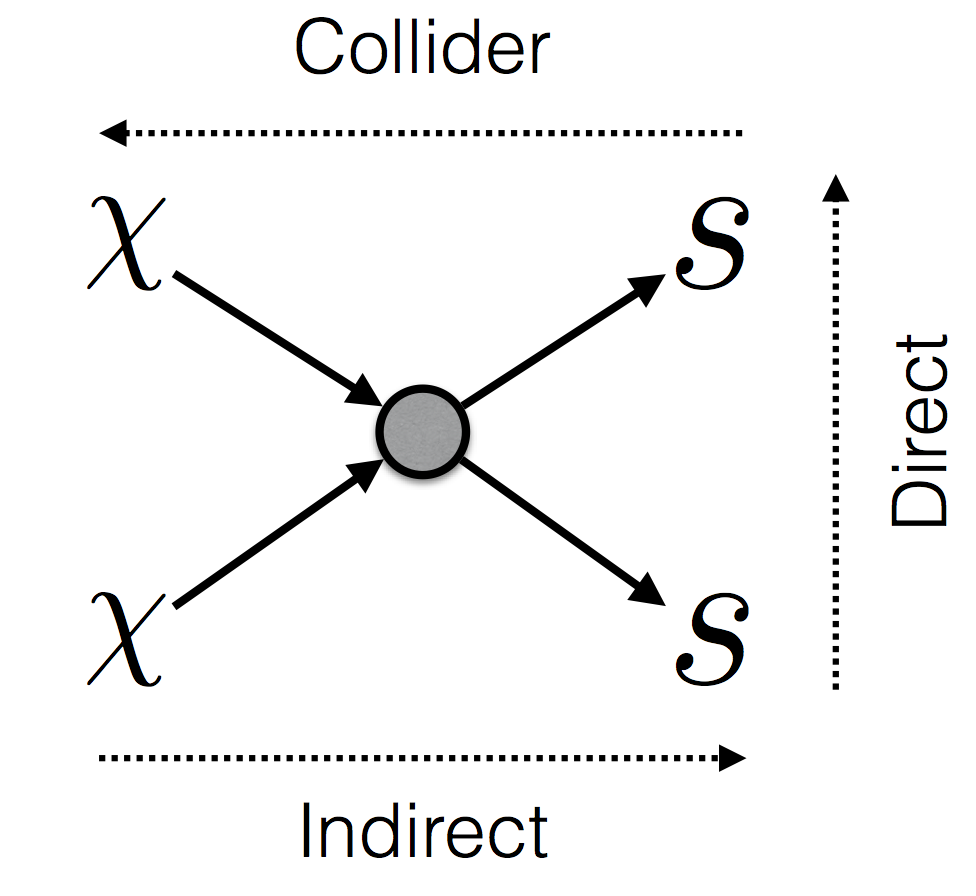
\includegraphics[width=0.65\textwidth]{images/3waystodetect/3waystodetect.pdf}
      \caption[3 Search Techniques]{
        The three general search techniques for dark matter.}
      \label{fig:3_searches}
    \end{figure}
    
    In collider searches, $ss \rightarrow \chi\chi$, standard model particles ($ss$) are collided within a detector, and the resulting particle fragments are measured by a slew of detectors~\cite{atlas,cms}.
    {\color{red}(You sometimes use capital S and sometimes lower-case s. ?? -orel)}
    These detectors include scintillation crystals with avalanche photodiodes and silicon strip detectors.
    Some of these detectors are within magnetic fields that curve charged particles, aiding in their measurement.
    Since the initial particles are accelerated to known energies, and the output fragment particles are well measured, searching for any break from conservation laws may hint at dark matter particles. 
    
    For direct searches, $\chi s \rightarrow \chi s$, sensitive particle detectors are built deep underground.
    When a WIMP impacts a nucleus within the detector, an observable signal can be produced.
    {\color{red}(Maybe rewrite slightly to say that you will give examples of the signal expected in each type of experiment below?  Maybe also consider listing  the experiments in bullets. ?? -orel)}
    Being underground shields the detectors from cosmic rays, which create background collisions that can mask WIMP signals.
    {\color{red}(Does the background mask the WIMP signal or mimic it?? -orel)}
    In liquid Xenon detectors, particle collisions in the liquid produce UV photons and electrons, which are used to infer the presence of WIMPS~\cite{direct_lux}.
    Cryogenic detectors use pucks of germanium and silicon to measure particle collisions.
    These collisions produce detectable ionization and phonon signals, which are used to classify the incident particle~\cite{direct_cdms}.
    Scintillation detectors are built with crystals like Titanium-doped Sodium Iodine.
    When an external particle collides with a nucleus of the crystal, the nucleus becomes excited, then relaxes by releasing a photon~\cite{direct_dama}.
    However, to date no substantial dark matter signal has been detected with these methods~\cite{direct_dm_detection}.
    
    For indirect searches, $\chi\chi \rightarrow ss$, astrophysical observations are analyzed for excess amounts of standard model particles, more than can be explained by known astrophysical processes.
    {\color{red}(You jumped a bit, first say you are looking for an excess in data from the centre of the galaxy and then state why. -orel ??)}
    This analysis searches for an excess of gamma rays, as the center of our galaxy is believed to host a dark matter halo.
    This spherical halo would allow for many $\chi\chi$ annihilations, producing gamma rays via: 
    
    $$\chi\bar{\chi} \rightarrow S\bar{S} \rightarrow \gamma\gamma$$

    where $S\bar{S}$ can be any quark or lepton particle-antiparticle pair ($t\bar{t}$, $s\bar{s}$, $e^{-}e^{+}$, etc).
    These different annhilation channels can produce different spectra of gamma rays, which will also vary based on the WIMP mass and cross section chosen.
    This is described further in Section \ref{dm_spectral}.

\FloatBarrier

\section{Galactic Center}
  
  {\color{red}(The structure of this section is strange. You start by giving 3 examples of the gamma-ray sources there. Then you describe only two of them in more detail, with some repetitions of the intro. I suggest you re-write. Maybe move the black hole to the intro and then give a short description of all three gamma-ray sources in their own sub-sub-sections. -orel ??)}

  The Galactic Center is a complex region of space, with many astrophysical sources of gamma rays.
  {\color{red}(Maybe help the reader understand you are listing a few sources of gamma rays from the GC? It reads a little clunky as it is, took me until I reached the end to understand you are giving examples (partly because of the word "also" in the middle). ?? -orel)}
  A disk of dust lies along the galactic plane, acting as an interaction medium for diffuse proton cosmic rays.
  Nearby supernova remnants also produce gamma rays as their expanding shells interact with ambient dust.
  The immediate area surrounding the Galactic Center contains a point-source gamma-ray emitter, although its mechanism is poorly understood.

  % black hole
  Through kinematic observations of nearby stars, it was deduced that the Galactic Center is home to a supermassive black hole, with a mass of \SI{4e6}{ \Msol{} }~\cite{sgra_massdist}.
  The Galactic Center is also a source of TeV gamma rays~\cite{gc_pointsrc_hess,gc_pointsource_hess2,gc_veritas_pointsource,gc_magic_pointsource}, though the mechanism that produces them is still under debate.
  One possibility is that the supermassive black hole accelerates protons to PeV energies, which then collide with local atoms to produce $\pi^0$s, which then decay into TeV gamma rays~\cite{gc_pevatron}.
  The second possibility suggests a nearby population of pulsar wind nebulae may be accelerating electrons, which then upscatter local photons to TeV energies~\cite{gc_pulsars}.
  While the Galactic Center is a source of gamma rays, the current generation of gamma-ray telescopes can only resolve it into a point source, due to their limited angular resolution~\cite{VeritasGCRidge2015,gc_pointsrc_hess}.
  {\color{red}(Why do you start the sentence with "while"? There is no conclusion to it. I assume you wanted to say that you think the GC is a complex source of gamma rays, originating from different areas in it, but that for now we only see a point source. You can say that, but be careful with the language (use "potentially"?). ?? -orel)}

  The disk of gas present in the galactic plane acts as an interaction medium for passing protons, both from nearby galactic accelerators and from extragalactic sources.
  The interactions between this disk of gas and protons produce $\pi^0$'s, which decay into $\gamma\gamma$ pairs~\cite{hess_gc_diffuse}.
  This emission is not modeled in this analysis, as atmospheric effects overwhelm any diffuse emission the residual skymaps\footnote{These residual maps are discussed in Section~\ref{subsec:likemax}.}.


\section{Indirect Dark Matter Search}
  For this analysis, it is necessary to understand how a terrestrial telescope can detect the presence of dark matter.
  Imaging atmospheric cherenkov telescopes like H.E.S.S., MAGIC, and VERITAS can indirectly search for dark matter.
  In these searches, these observatories detect gamma rays that are emitted when two dark matter particles annihilate.
  Because the rate of annihilation depends on the local dark matter density, the radially-dependent structure of dark matter halos also affects the analysis.
  {\color{red}(It doesn't affect the analysis, it affects the gamma-ray emission rate. -orel ??)}

  \subsection{Dark Matter and Gamma Rays}
    Primarily, indirect searches focus on annihilating WIMPs, as the predicted decaying WIMP produces a lower flux of standard model particles than annihilation.
    WIMPs may annihilate into any standard model particle-antiparticle pair, but most studies examine a WIMP annihilating into a quark-antiquark pair, or a pair of gamma-ray photons.
    For example, two annihilating WIMPs may produce a $t\bar{t}$ pair, which then decays into $W^+bW^-\bar{b}$~\cite{pdg2016}.
    Alternately, other pairs may be produced, like  $b\bar{b}$, $c\bar{c}$, $W^+W^-$, $u^+u^-$, or $\tau^+\tau^-$.
    These different annihilations produce different spectra of final gamma rays.
    The final spectrum of gamma rays used in this analysis is calculated in Section~\ref{dm_spectral}.
  
  \subsection{Dark Matter Halo Structure}\label{dm_spatial}
    
    {\color{red}(Why don't you merge this section with 3.3.4? It feels a little empty as it is. ?? -orel)}
    
    Observations allow most galactic dark matter halos to be modeled using a class of similar density profiles.
    A currently favored profile is the Einasto profile~\cite{einastoprofile1,einastoprofile2}.
    This profile describes the mass-density of dark matter at a distance $r$ from the halo center, $\rho(r)$.
    The Einasto profile is described by Equation~\ref{eqn:einasto}:

    \begin{equation} \label{eqn:einasto}
      \rho_{\textrm{DM}} \left( r \right) = \rho_{s} Exp \left( - \frac{2}{\alpha} \left( {\left( \frac{r}{r_s} \right)}^{\alpha} - 1 \right) \right) \;\; .
    \end{equation}
    
    
    In Equation~\ref{eqn:einasto}, $r_s$ is the scale radius of the halo, which specifies how wide the dark matter halo is.
    The parameter $\rho_s$ is the scale density, the dark matter density at the scale radius.
    The parameter $\alpha$ is the power of the density profile's slope.
    A larger $\alpha$ results in smaller dark matter densities above and below the scale radius $r_s$.
    In the model, the parameter $\alpha$ is fixed to 0.17, and $r_s$ is fixed to \SI{15.14}{kpc}.
    {\color{red}(Maybe reverse the order? You say that $\alpha$ and $r_s$ are from best fit values, then how $r_s$ is calculated. So after that you can give the alpha value and say that both are kept fix in your analysis or in the model. ?? -orel)}
    Both $\alpha$ and $r_s$ are from the best fit values of the Aq-A-1 simulation in Table 2 of Ref.~\cite{mw_halo_params}.
    The $r_s$ parameter is calculated via $r_s=r_{-2}=15.14\:\textrm{kpc}$, where $r_{-2}=\frac{11.05}{h_{73}}\:\textrm{kpc}$ (in Ref.~\cite{mw_halo_params}, Table 2) and $h_{73}=0.73$ from Section 2.1 in Ref.~\cite{mw_halo_params}.
    The distance to the galactic center is known to be $r_\odot=8\:\textrm{kpc}$~\cite{gc_distance_1,gc_distance_2,gc_distance_3}.
    The assumed Milky Way mass profile has a mass density of $\rho_\odot = 0.4\:\frac{\textrm{GeV}}{\textrm{cm}^3}$~\cite{local_dm_density,direct_dm_astrophysical_uncertainties}.
    Since $r_\odot$ and $\rho_\odot$ are known, then in Equation~\ref{eqn:einasto} the dark matter density at the scale radius $\rho_s$ is derived to be \SI{0.12}{\GeV\per\cm^3}.
    With these values, the Einasto profile in Equation~\ref{eqn:einasto} is shown in Figure~\ref{fig:gchalo_density}.
  
    \begin{figure}[ht]
      \centering
      \includegraphics[width=0.95\textwidth]{images/halo/gc_einasto_profile.pdf}
      \caption[Galactic Center Einasto Halo Density]{
        Mass density of the Einasto dark matter halo (Equation~\ref{eqn:einasto}) used in this analysis.
        The bottom x axis shows the angle from the Galactic Center, while the top x axis shows the distance in kiloparsecs.
        \CaptionBlankLine
        }
      \label{fig:gchalo_density}
    \end{figure}

    Other density profiles exist, but in this analysis only the Einasto profile is considered.
    Most simulations show that density profiles should terminate in a sharp peak at $r=0$, but observations of dwarf galaxies instead favor a flat core within a given radius~\cite{flores1994observational,CoreVsCusp}.
    This may be due to the presence of baryons in this core region, which can diffuse the central cusp of WIMPs into a core-like shape~\cite{corecusp_baryondiffuse1,corecusp_baryondiffuse2}.
    As this flat core occurs in the inner-most region covered by the gamma-ray observations {\color{red}in this analysis}, the choice of a cuspy or cored dark matter halo can have a significant impact {\color{red}on this analysis} {\color{red}(in this analysis, vs on this analysis?? -orel)}.
    Specifically, if the dark matter halo follows a cored profile when using a cuspy halo model, then any derived upper limits on the dark matter cross section would be different.
    For simplicity, only a cuspy halo is used in this thesis.
    
    When choosing which dark matter target to observe with a gamma-ray observatory, knowing the gamma-ray brightness of different sources can be useful.
    This Einasto density profile can be integrated to calculate this gamma-ray brightness, independent of the WIMP model being searched for.
    For annihilating dark matter, $\rho_{\textrm{DM}}\left(r\right)^2$ must be integrated along the line of sight.
    Equation~\ref{eqn:dmflux} can be used to calculate the amount of gamma rays produced by these annihilations.
    
    \begin{equation}\label{eqn:dmflux}
      \frac{ d\Phi }{ dE d \Omega } = \frac{ \left \langle \sigma v \right \rangle }{8 \pi m_\chi^2} \frac{dN_{\gamma}}{dE} \int \rho^2 dl
    \end{equation}
    
    In this equation, the photon flux $\Phi$ is the number of gamma rays detected per $\textrm{area}\times\textrm{time}$.
    The velocity-averaged cross section of the dark matter candidate is $\left \langle \sigma v \right \rangle$.
    Velocity-averaging is used because the cross section is velocity dependent, and the WIMPs that pass through a volume of space will have a distribution of velocities~\cite{wimp_veldist}.
    The spectrum of photons produced by a single $\chi\chi$ annihilation is $\frac{dN_{\gamma}}{dE}$.
    The density integral in Equation~\ref{eqn:dmflux} is often calculated separately, as in Equation~\ref{eqn:jfactor}, and is referred to as the $J$ factor,

    \begin{equation}\label{eqn:jfactor}
      J = \int \rho^2 dl \;\; .
    \end{equation}

    The $J$ factor is sometimes separately calculated to compare the relative gamma-ray brightness of different dark matter halos, which is a function of both dark matter density and observing distance.
    The Einasto density in Equation~\ref{eqn:einasto} can be integrated to calculate the $J$ factor at various radii, which is shown in Figure~\ref{fig:gchalo_jfactor}.
    The values in this figure are calculated using an integration radius of \ang{0.01}.
    {\color{red}(What does the integration radius mean here exactly?? It is not entirely clear from this discussion. -orel)}
    This J-factor profile then forms the spatial component of the dark matter halo, $M_{s,\textrm{halo}}$, used in Chapter~\ref{chapter:analysis}.
    The J-factor is shown in a two-dimensional plot in Figure~\ref{fig:halojfactor}.
    
    \begin{figure}[ht]
    \centering
      \includegraphics[width=0.95\textwidth]{images/halo/gc_einasto_jfactor.pdf}
      \caption[Galactic Center Einasto Halo Jfactor]{
        J-factor profile as a function of angle from the Galactic Center, calculated via Equation~\ref{eqn:jfactor} with the Einasto density profile in Equation~\ref{eqn:einasto}.
        J-factor values are calculated with an integration angle of \ang{0.01}.
      }
      \label{fig:gchalo_jfactor}
    \end{figure}
    
  
  \begin{figure}[ht]
    \centering
    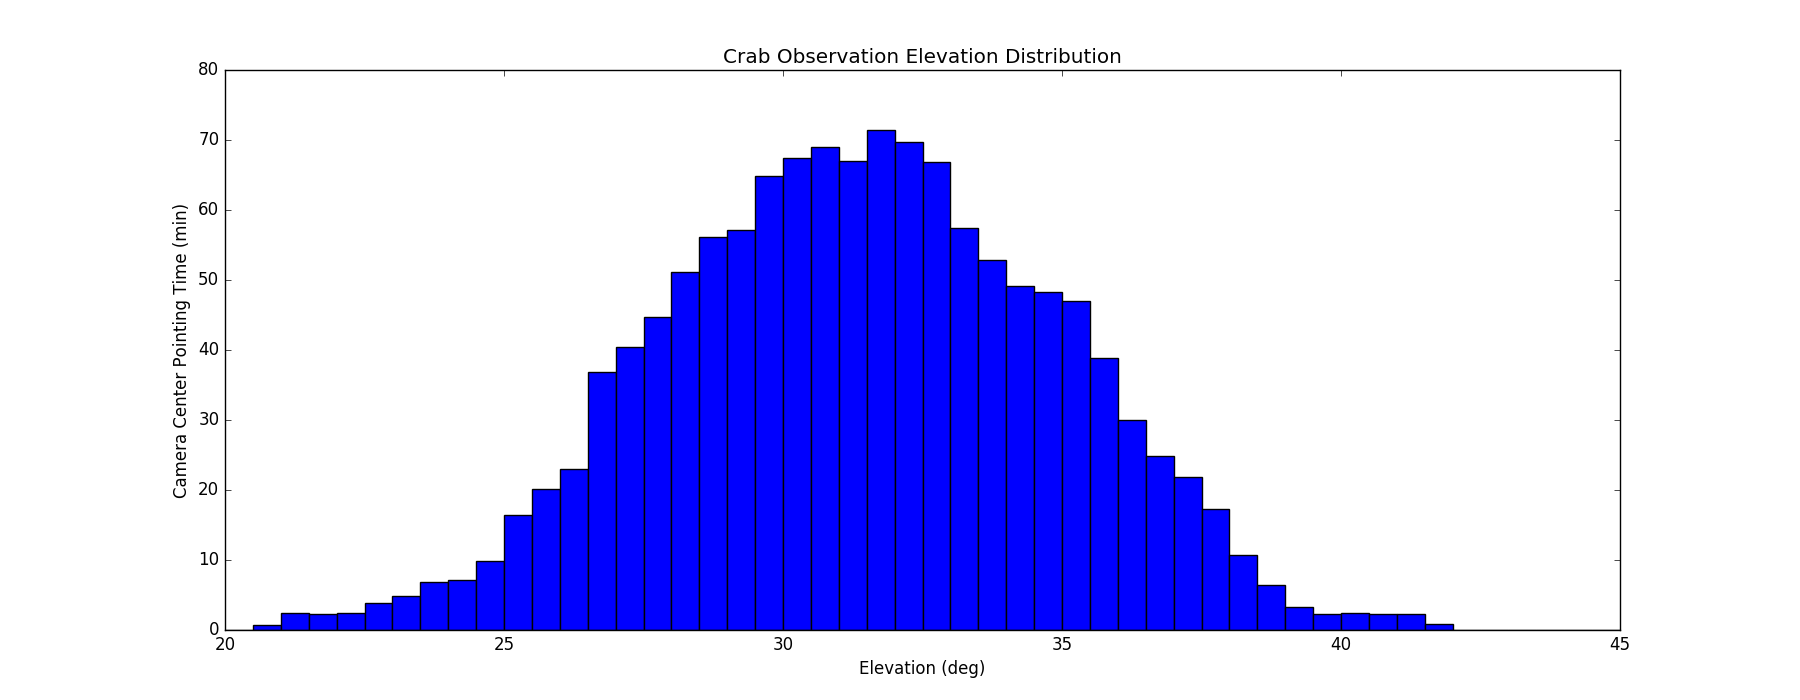
\includegraphics[width=0.95\textwidth]{images/halo_flux/plot.pdf}
    \caption[Galactic Center Halo J-factor Skymap]{
      J-factor of the dark matter halo model used in this analysis.
      The green circles indicate the different observation regions.
      Note this is showing the same model as Figure~\ref{fig:gchalo_jfactor}, except here the J-factor axis is linear instead of logarithmic.
      The black corners are from the halo model only being calculated out to a radius of \ang{3}, since there are no observations that extend past that.
    }
    \label{fig:halojfactor}
  \end{figure}

  {\color{red}(This is not connected enough to the previous paragraphs. Maybe put it in its own sub-sub-section with a short intro?? -orel)}
  More exotic WIMP models may slightly alter the gamma-ray brightness of the dark matter halo, compared to the previously mentioned WIMP model.
  For example, if dark matter WIMPs have an attractive force between them, their effective annihilation cross section is enhanced, increasing the gamma-ray emission from the halo.
  This effect is called Sommerfeld Enhancement~\cite{sommerfeld}.
  The dark matter model searched for in this thesis does not include this effect.
  % originally from http://inspirehep.net/record/1286230/files/Thesis-2009-Nierop.pdf
  % from http://www.pnas.org/content/112/40/12264.full.pdf
    
  
  \FloatBarrier
  
    
  \subsection{Spectrum of Gamma Rays from Dark Matter}\label{dm_spectral}
    In order to calculate the gamma-ray brightness of the dark matter halo, the produced spectrum from each WIMP annihilation must be known.
    Each WIMP annihilation can have distinct outcomes (each producing different pairs of particles), referred to as annihilation channels.
    WIMPs may annihilate directly into two gamma rays (the $\gamma\gamma$ channel), or may instead produce a quark-antiquark pair ($b\bar{b}$, $t\bar{t}$, ...), a lepton-antilepton pair, or almost any other standard model particle-antiparticle pair.

    Non-gamma-ray annihilation channels may still indirectly produce gamma rays as the original particle pair decays.
    Many standard model particle-antiparticle annihilations also result in a mix of annihilation channels, so WIMPs may also have this feature.
    {\color{red}(What do you mean by these mixing channels?? -orel)}
    Mixing channels requires multiple dark-matter halo models however, which is beyond the scope of this single halo analysis.
    {\color{red}(Why do these mixing channels require multiple dark-matter halo models?? -orel )}
    The software package CLUMPY~\cite{CLUMPYcode} is used to calculate the gamma-ray spectra for each annihilation channel.
    The spectral models that CLUMPY uses are based on the tables in the PPPC 4 DM ID~\cite{pppc4_dm_spectra}.
    For this analysis, only the $b\bar{b}$ annihilation channel is considered.
    Figure~\ref{fig:chichi_spectrum} shows the resultant spectra from the single annihilation of two WIMPs.
    {\color{red}(You should say how these spectra were calculated (using clumpy?). Also in the figure caption. Are these detailed simulations of the production and then decay of bb?? -orel )}
    Each line shows the spectrum from a different initial WIMP mass.

    \begin{figure}[ht]
      \centering
      \includegraphics[width=0.95\textwidth]{images/spectra/chichi_spectrum.pdf}
      \caption[Single Annihilation Spectra]{
        Resultant photon spectra from a single annihilation of WIMP particles.
        Each colored line represents a different WIMP mass.}
      \label{fig:chichi_spectrum}
    \end{figure}


    These spectra can be combined with the J factor Equation~\ref{eqn:jfactor} to calculate Equation~\ref{eqn:dmflux}: how many gamma rays are produced by the halo\footnote{
      These spectra are then used as the spectral component $M_{\textrm{e,halo}}$ for the dark matter halo model in the likelihood analysis in Equation~\ref{eqn:dmmodel}, detailed further in Section~\ref{subsec:dmhalomodel}.
    }.
    {\color{red}(many gamma rays are produced by the halo (Not sure if I would point to equation 6.21. I would show and explain the equation here as this chapter describes the physics needed to understand the thesis. This happened previously in the thesis again. ?? -maria,orel ))}

    \FloatBarrier
    
    
\section{Atmospheric Showers}

  When a particle strikes an atom of Earth's atmosphere at GeV or higher energies, it sets off a cascade of energetic particles called an air shower~\cite{Bethe1934,Klein1999}.
  When the primary particle is composed of one or more hadrons, like a proton or Iron atom, it creates a hadronic shower.
  When the primary is a gamma ray or a charged lepton, it creates an electromagnetic shower.
  Electromagnetic showers produce a cascade of $e^{\pm}$s and $\gamma$'s, where each successive generation of particles tends to have more particles but less energy per particle than the last.
  To start the shower, the primary gamma ray will interact with an atmospheric atom, producing an $e^{-}e^{+}$ pair, each with roughly half the primary gamma ray's energy, as shown in Figure~\ref{fig:emcascade}.
  The $e^{-}$ and $e^{+}$ emit bremstrahlung photons, and incite the atmosphere to emit Cherenkov photons,.
  Cherenkov photon production is discussed further in Section~\ref{sec:cherenkov}.
  The higher-energy bremstrahlung photons then pair produce $e^{-}e^{+}$, which go on to produce more bremstrahlung and cherenkov photons.
  As each newly created particle has less energy than its parent particle, eventually the particles in the shower don't have enough energy to produce additional child-particles.
  When electrons have around \SI{80}{MeV} or less of kinetic energy, energy losses due to ionization begin to dominate~\cite{pdg_2014}.

  \begin{figure}[ht]
    \centering
    \includegraphics[width=0.95\textwidth]{images/cascade_diagram/feynman/cascade.pdf}
    \caption[Electromagnetic Cascade]{
      Diagram of the first few generations of an electromagnetic cascade as it decends downwards through the atmosphere, layered by interaction generation~\cite{ellis2017tikz}.
      At the top of the diagram, $\gamma{}_o$ is the initial astrophysical gamma ray.
      \CaptionBlankLine
    }
    \label{fig:emcascade}
  \end{figure}

  Of all detected air showers, \nicetilde{}99\% are due to protons and electrons, and not gamma rays.
  {\color{red}(Maybe first say how a hadronic shower looks like and what it is and only then talk about the gamma-hadron separation?? -orel)}
  Understanding the differences between hadronic and electromagnetic showers is useful for removing unwanted proton events and preserving gamma-ray events within the reconstruction method, sometimes referred to as gamma-hadron separation.
  {\color{red}(You haven't really defined what an event is. Also, I would finish the sentence after gamma-ray events and in the next sentence simply say that this process of selecting gamma-ray events is usually referred to as gamma-hadron separation. ?? -orel)}
  Hadronic showers start with a primary \nicetilde TeV proton $p_{cosmic}$ that interacts with an atmospheric proton $p_{atmo}$.
  The proton-proton collision then produces a set of pions, as in Equation~\ref{eqn:protoncollision}, as well as other particles (`$X$') whose production rates vary with available interaction energy.
  {\color{red}(The pp interaction doesn't always produce pions, right?? First you should talk in general about Hadronic air showers and then focus on those which look like gamma rays. Why don't you start with general lines, saying that many particles are produced at different rates and in different directions, mention how that would look like and then say that some of those particles are $\pi_0$ which produce electromagnetic showers. -orel )}
  
  \begin{equation}\label{eqn:protoncollision}
    p_{cosmic} + p_{atmo} \rightarrow \pi^+ + \pi^+ + \pi^0 + ...
  \end{equation}
  
  The interaction produces $\pi^+\pi^+\pi^0$, each with roughly \nicetilde $\frac{1}{3}$ of the initial proton's energy.
  {\color{red}(You discussed this decay to gammas 3-4 times before, why show the diagram only now?? -orel)}
  This $\pi^{0}$ decay is shown in Figure~\ref{fig:feynman_pi0}.
  
  \begin{figure}[ht]
    \centering
    \includegraphics[width=0.5\textwidth]{images/feynman_particles/pion_gamma.pdf}
    \caption[Feynman Diagram of $\pi^{0}$ Decay]{
      Feynman diagram of a $\pi^{0}$ decaying into two photons.
      \CaptionBlankLine
    }
    \label{fig:feynman_pi0}
  \end{figure}

  \begin{figure}[ht]
    \centering
    \includegraphics[width=0.5\textwidth]{images/feynman_particles/pionplus.pdf}
    \caption[Feynman Diagram of $\pi^{+}$ Decay]{
      Feynman diagram of $\pi^{+}$ decaying into a lepton pair.
      \CaptionBlankLine
    }
    \label{fig:feynman_piplus}
  \end{figure}
  
  % see here for neutron: https://en.wikipedia.org/wiki/Cosmic_ray
  The $\pi^{+}$ and $\pi^{-}$ can travel far in the tranverse direction, away from the main axis of the primary particle, then decay into $\mu^{+}\nu_{\mu}$ and $\mu^{-}\bar{\nu}_{\mu}$ pairs, respectively.
  The $\pi^{+}$ decay is shown in Figure~\ref{fig:feynman_piplus}.
  The $\pi^{0}$ quickly decays into pair of gamma rays, each of which then start their own electromagnetic shower.
  {\color{red}(The decay itself was mentioned a few lines back, should rewrite this and combine so not to repeat too much. ?? -orel)}
  The $\pi^{+}$ and $\pi^{-}$ have longer decay times ($\pi^{\pm} \rightarrow $\SI{3e-8}{s} vs $\pi^{0} \rightarrow $\SI{9e-17}{s}~\cite{pdg_2014}), allowing them to carry energy farther away from the central shower axis.
  Both of these effects create sub-showers farther away from the primary particle axis, which tends to cause hadronic showers (and their resulting Cherenkov images, discussed in Section \ref{sec:cherenkov}) to be wider than a purely electromagnetic shower of the same length. 
  
  In Figure~\ref{fig:gamma_vs_proton_airshower}, the differences between a gamma-ray shower and a proton shower are shown.
  The gamma-ray shower on the left has most of its particles along the veritical core of the shower, while the proton shower has particles spread out in a wider, fan-like shape.
  The initial energies were chosen as such because a \SI{1}{TeV} proton will on average divest $\frac{1}{3}$ of its energy to the $\pi^{0}$.
  Since these two showers start with the same amount of available energy, they produce a similar amount of Cherenkov light.
  {\color{red}(You haven't discussed the Cherenkov light yet, so it's a little weird to mention this ratio here. Maybe talk about Cherenkov light earlier? Also, why is the last paragraph its own paragraph?? -orel)}

  This $\pi^{0}$ then decays into the electromagnetic sub-shower faintly visible in the interior of the proton shower.
  The net effect is that, when compared to a gamma ray, a proton must start with 3 times the energy to produce a similar amount of Cherenkov photons, which are distributed in a wider pattern.

  \begin{figure}[ht]
    \centering
    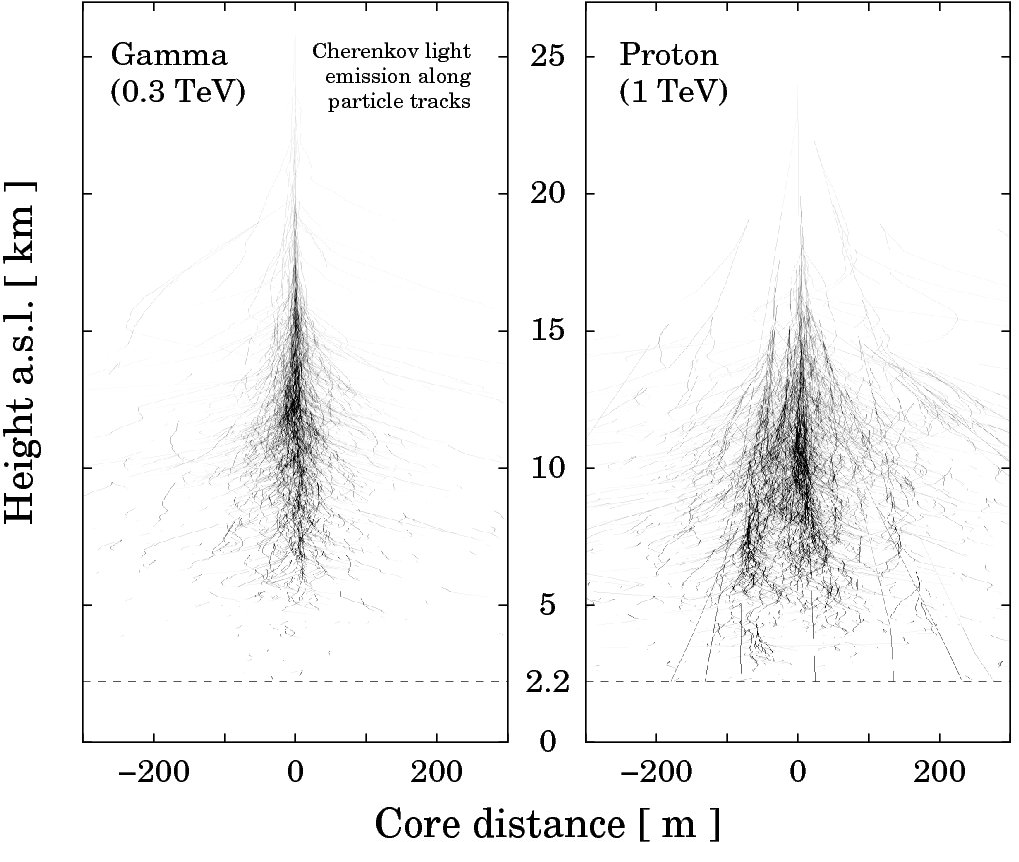
\includegraphics[width=0.95\textwidth]{images/showers_gamma_proton}
    \caption[Gamma Ray and Proton Showers]{
      A gamma ray shower alongside a proton shower~\cite{Bernlohr2008149}.
    }
    \label{fig:gamma_vs_proton_airshower}
  \end{figure}
  
  \FloatBarrier

  \subsection{Cherenkov Photons}\label{sec:cherenkov}

  Within atmospheric showers, any charged particles travelling at velocity $v > c_{atmosphere}$, where $c_{atmosphere}$ is the speed of light in the atmosphere, will induce the atmosphere to produce Cherenkov photons~\cite{cherenkov}.
  From a single charged particle of constant velocity, Cherenkov photons form a conical wavefront shown in Figure~\ref{fig:cherenkovangle}, similar to a sonic boom shockwave or the wake produced when a boat travels faster than the speed of the waves.

  \begin{figure}[ht]
    \centering
    \includegraphics[width=0.27\textwidth]{images/cherenkov_angle/cherenkovangle.pdf}
    \caption[Chernekov Emission Angle]{
      Cherenkov light (blue arrows) is emitted at angle $\theta$, relative to the charged particle z's path.
    }
    \label{fig:cherenkovangle}
  \end{figure}

  Cherenkov photons are produced at an angle $\theta$ relative to the charged particle's path, determined by the index of refraction of the medium $n$, the speed of the charged particle $v$, and the speed of light in the medium $c$, as in Equation~\ref{eqn:cherenkovangle}.

  \begin{equation}\label{eqn:cherenkovangle}
    \theta = ArcCos \left ( \frac{c}{n \; v} \right )
  \end{equation}
  
  For the gamma-ray showers used in this analysis, the cherenkov angle $\theta$ is \nicetilde\ang{1}.
  {\color{red}(Is it only for the gamma-ray showers this angle?? -orel)}
  % showers are 10km up, light pool on ground is 130m diameter, \theta = ArcSin(130/10000) * 180 / pi = 0.73deg ~ 1deg

  However in an atmospheric shower, the number and distribution of charged particles and their velocities, as well as energy losses, tend to smear the theoretically-clean Cherenkov cones into a diffuse pool of light on the ground, shown in Figure~\ref{fig:lightpool}.

  \begin{figure}[ht]
    \centering
    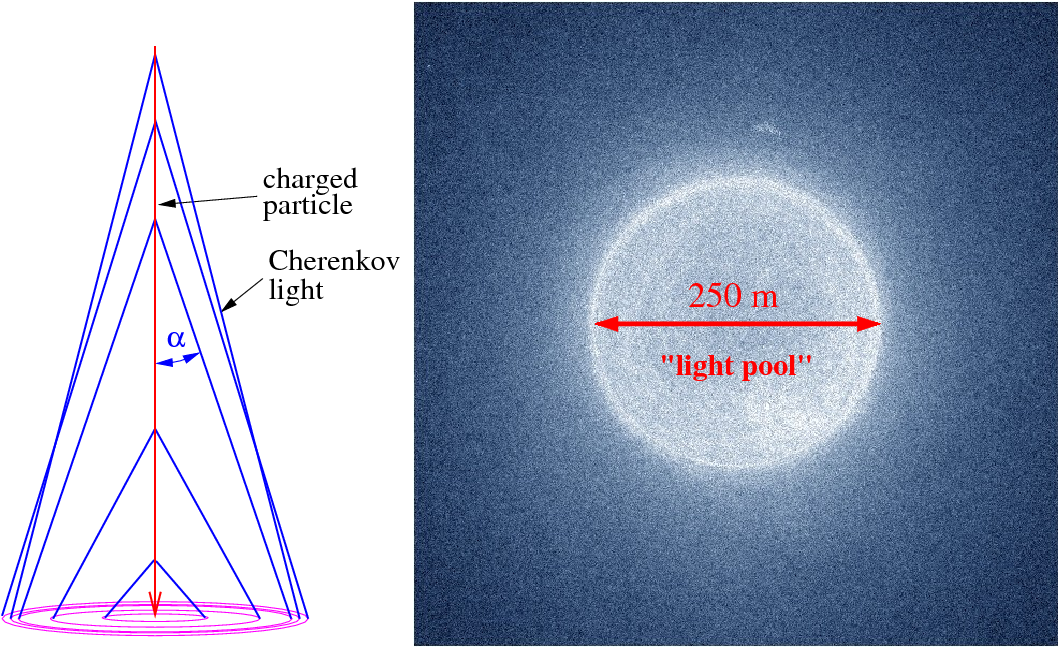
\includegraphics[width=0.85\textwidth]{images/lightpool/lightpool.pdf}
    \caption[Chernekov Light Pool]{
      Cherenkov light from a gamma ray shower illuminating the ground.
      Due to the changing atmospheric density, the cherenkov angle changes as the electromagnetic shower decends (Left), concentrating the emitted light into a ring-like pool (Right).
      The initial gamma ray had an energy of \SI{1}{\TeV}.
      Figure is from Ref.~\cite{Voelk}.
    }
    \label{fig:lightpool}
  \end{figure}
  
  The spectrum of photons produced by the Cherenkov effect can be calculated with the Frank-Tamm formula~\cite{franktamm1,franktamm2} in Equation~\ref{eqn:franktamm},
  
  \begin{equation}\label{eqn:franktamm}
    \frac{dE}{dx\,d\omega}=\frac{(ze)^2 \, \omega}{c^2} \left ( 1 - \frac{c^2}{v^2 \;\epsilon(\omega)} \right )
  \end{equation}
  
  where $E$ is the energy emitted as Cherenkov radiation, $x$ is the length of the charged particle path, $ze$ is the charge of the particle, $\omega$ is the emitted Cherenkov photon frequency, $c$ is the speed of light (phase velocity) in the medium, $v$ is the speed of the particle, and $\epsilon(\omega)$ is the frequency-dependent permittivity.
  The UV- and visible-spectrum Cherenkov photons are then imaged and recorded by the VERITAS observatory.
  
  \begin{figure}[ht]
    \centering
    \includegraphics[width=0.75\textwidth]{images/CherenkovReactor/cherenkovreactor.eps}
    \caption[Chernekov Light from a Reactor]{
      Blue Cherenkov light in the Advanced Test Rector core, at the Idaho National Laboratory~\cite{cherenkovreactor,atrlab}.
    }
    \label{fig:cherenkovreactor}
  \end{figure}
  
  In Figure~\ref{fig:cherenkovreactor}, a visible example of Cherenkov photons is shown, produced in the Advanced Test Reactor at the Idaho National Laboratory.
  Neutrons emitted by the reactor collide with atoms in the water, freeing some electrons with enough kinetic energy to travel faster than the speed of light in water.
  These superluminal-in-water electrons then create the blue Cherenkov photons imaged here.
  
